\documentclass[conference]{IEEEtran}
\IEEEoverridecommandlockouts
\usepackage{cite}
\usepackage{amsmath,amssymb,amsfonts}
\usepackage{algorithmic}
\usepackage{graphicx}
\usepackage{textcomp}
\usepackage{xcolor}
\usepackage{booktabs}
\def\BibTeX{{\rm B\kern-.05em{\sc i\kern-.025em b}\kern-.08em
    T\kern-.1667em\lower.7ex\hbox{E}\kern-.125emX}}
\begin{document}
\title{Bias in AI: Implementation Project}
\author{\IEEEauthorblockN{fsdn71}
\IEEEauthorblockA{\textit{Department of Computer Science} \\
\textit{University of Durham}\\
Durham, United Kingdom \\
fsdn71@durham.ac.uk}
}
\maketitle

\section{Project Proposal}
\subsection{Outline}
The Adult Income dataset is a subset of the U.S. Census database, and is widely accepted as an accurate and predictive representation of the living circumstances of the U.S. population. It contains demographic, financial and employment-related information in both continuous and categorical forms, making it useful for training machine learning-based algorithms to predict various socio-economic features. However, it has been found to contain significant biases among race and gender attributes, persisting across multiple variables\cite{DBLP:journals/corr/abs-1908-09635}. Therefore, this presents a suitable challenge for bias countermeasures to reduce bias shown in predictive models trained on the data. This project is proposed to analyse and implement state-of-the-art anti-bias methods on a classifier predicting whether an adult's annual income is over $\$50,000$, given data on employment class, capital flow and household attributes.
\subsection{Motivation}
The existence of gender and racial biases in the microdata is not unexpected - arising predominantly from historical imbalance in public policy. However, models which predict income or demographic variables can introduce or perpetuate bias, facilitating discrimination towards real-life individuals, when the outputs of the model are used to inform decisions on lending, hiring and other areas. Developing models which ensure fair outcomes for individuals is therefore a positive contribution to society, and one that this project aims to reproduce.

The Adult Income dataset is also appealing as an implementation project for fairness because of its wide coverage of individuals - the Census features every household in the U.S. Other datasets, such as those relating to online services such as Wikipedia or YouTube or educational outcome microdata, feature smaller subsets of the population, often with characteristics significantly different than the general population. The Census dataset is a suitable representation of the population, and includes weights for individual records, allowing a user to extrapolate directly onto the population. This means that algorithms applied onto the dataset will have some accurate insight into the biases present in the population as a whole, as well as how these could be altered with fairness regulation.
\subsection{Adversarial Learning}
The Adult Income dataset is well-established across the sub-fields of machine learning,with it being used to benchmark many different approaches to algorithmic fairness In \emph{One-Network Adversarial Fairness}, Adel et al. outline a framework for explicitly discouraging discriminative behaviour within classification models\cite{Adel_Valera_Ghahramani_Weller_2019}. This is achieved by mandating that the inputs to a classifier be modified by a separate model (a neural network in the paper), such that an adversary cannot identify the sensitive attribute. This method has been selected as the fairness measure to implement due to its novelty, strong previous results and prior application on the dataset. Furthermore, as found in \cite{DBLP:journals/corr/abs-1802-06309}, a representation-generation process that is accurate and unbiased on one task can be used as input to other predictive models using the same underlying data, improving fairness and retaining utility.
\subsection{Planning}
The implementation will involve the following steps:
\begin{enumerate}
    \item Dataset pre-processing: decoding categorical features into one-hot representation, normalising continuous features.
    \item Dataset analysis: producing descriptive statistics, broken down by sensitive attribute, to investigate the existing bias in the dataset, using Python libraries such as NumPy, Pandas and Plotly for data handling and visualisation.
    \item Conventional implementation: using the TensorFlow\cite{tensorflow2015-whitepaper} library, a neural network model comparable to the model used in \cite{Adel_Valera_Ghahramani_Weller_2019} will be trained and tested on partitions of the dataset. Bias and utility will be reported.
    \item Adversarial implementation: The model described in \cite{Adel_Valera_Ghahramani_Weller_2019} will be implemented and applied to the conventional implementation training process. Changes in bias and utility will be reported, in comparison to the conventional algorithm.
\end{enumerate}
The end result of the project will be a detailed analysis of existing bias in each of: U.S. survey microdata labels, outputs from an unconstrained neural network model, outputs from a model trained with adversarial fairness constraints. In addition, an investigation into the utility-bias trade-off within the fairness methods applied.
\section{Project Projects}
The implementation follows four major steps: analysis, conventional implementation and implementation of the adversarial model.
\subsection{Analysis}
The dataset contains a number of categorical features - these were transformed into one-hot encoded variables. The dataset does not contain null values, so no filtering was necessary. The sensitive attribute was selected as the intersection of race and gender - however, race was limited to White/Non-white values in order to keep the number of samples within each intersection similar. Additionally, when one-hot encoding categorical variables, categories with coverage of than $0.1\%$ of the microdata were removed. The implementation notebook contains four tables, showing descriptive statistics for categorical and continuous variables for each demographic subgroup. All statistics and graphs are calculated using the census weights matched to the $1994$ U.S. population.

The dataset shows significant bias in favour of both men and White individuals inclusively. Figure \ref{fig:fin_bias} shows the existing disparities in capital gains, loss and the high-income indicator, with the mean value for each subgroup as a percentage of the mean value for the population. It is clear that while bias exists along both racial and gender axes, gender-based bias is more severe. In addition, the distributions of continuous variables within demographic subgroups are different and may offer some explanation: Figure \ref{fig:hour_bias} shows the quantiles of weekly labour hours for each subgroup, indicating that the overall disparities are not caused by differences in the percentage working $40$ hours (the median), but by the comparatively larger and fewer percentages among non-white or female individuals working low ($20$) hours and high ($60$) hours, respectively.

\begin{figure}[h]
    \centering
    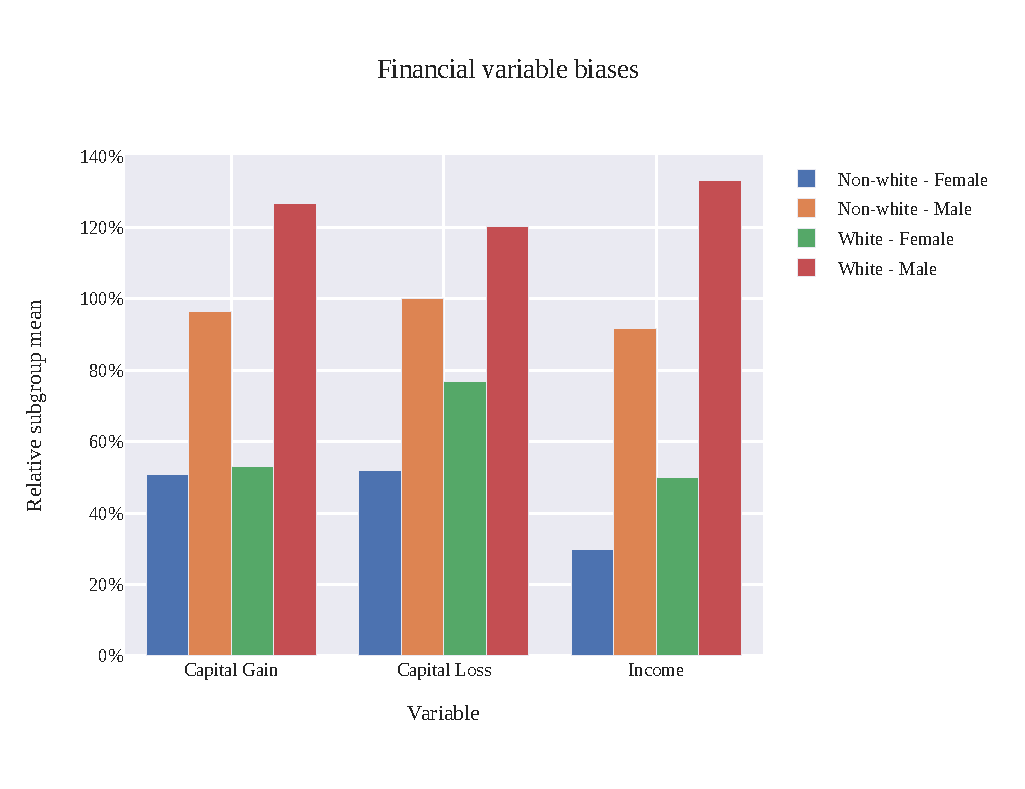
\includegraphics[width=0.5\textwidth]{images/fin_bias.pdf}
    \caption{Bias in financial variables}
    \label{fig:fin_bias}
\end{figure}

\begin{figure}[h]
    \centering
    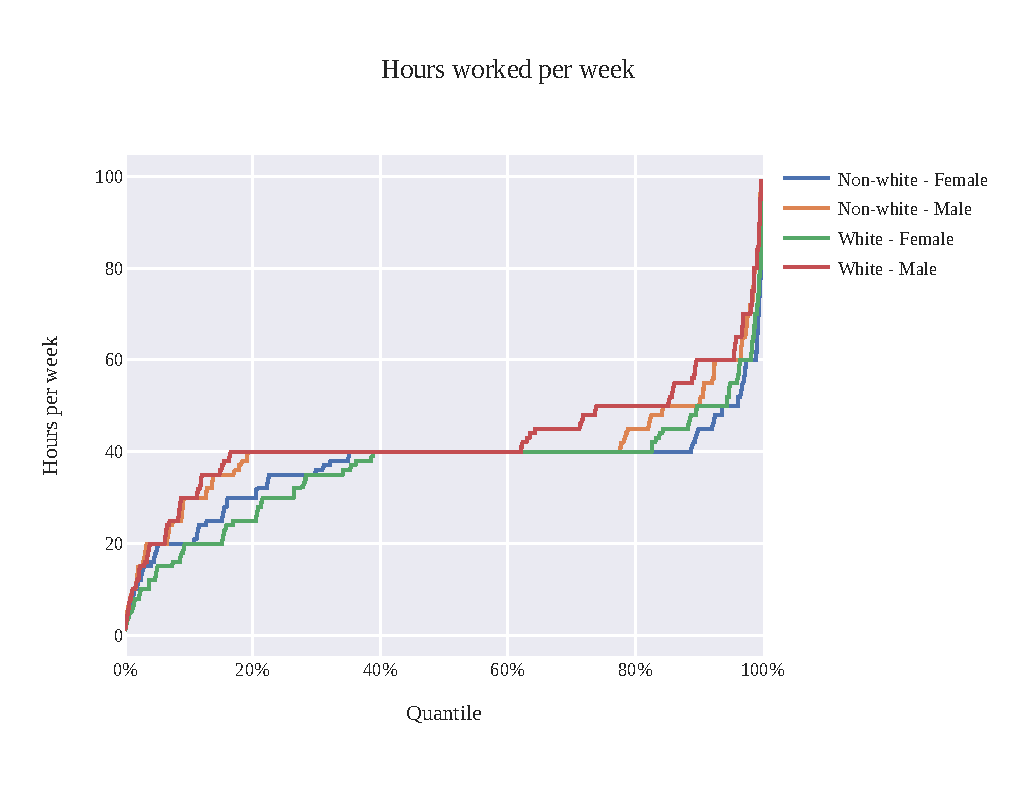
\includegraphics[width=0.5\textwidth]{images/hours_bias.pdf}
    \caption{Disparities in labour among subgroups}
    \label{fig:hour_bias}
\end{figure}

\subsection{Conventional Implementation}
After dataset pre-processing, we obtain three arrays of length $32,561$. These are $X$, the features ($79$ features), $S$, the sensitive attributes ($4$ features) and $Y$, the labels ($1$ label). These are split into training, validation and testing partitions (with ratio $80:10:10$).

The modelling approach taken is a standard deep neural network, consisting of two fully-connected layers (of size $64$ and $16$, respectively), each prepended with a dropout operation ($p=0.05$), and a final output with sigmoid activation. Table \ref{tab:conv_arch} shows the architecture of the model. The total number of parameters is $6,177$.

\begin{table}
    \caption{Conventional model architecture}
    \label{tab:conv_arch}
    \centering
    \begin{tabular}{llll}
        \toprule
        Index &        Name &        Type &         Shape \\
        \midrule
        0 &     input\_8 &  InputLayer &  [(None, 79)] \\
        1 &    dense\_21 &       Dense &    (None, 64) \\
        2 &  dropout\_14 &     Dropout &    (None, 64) \\
        3 &    dense\_22 &       Dense &    (None, 16) \\
        4 &  dropout\_15 &     Dropout &    (None, 16) \\
        5 &    dense\_23 &       Dense &     (None, 1) \\
        \bottomrule
    \end{tabular}
\end{table}
\bibliography{report.bib}
\bibliographystyle{IEEEtran}

\end{document}
